
\chapter{Graphing}
\section{Objectives}

\begin{enumerate}
    \item To learn to plot graphs using (i) a pencil and graph paper, (ii) Microsoft Excel, and (iii) Python.
\end{enumerate}

\section{Introduction}
Before you begin, read the article on graphing by Christopher Deacon. You don't need to grasp all the points in it right way, but as you grow in experience you will appreciate them.

\section{Graphing using pencil and graph paper}
Graphing, like many other scientific activities, begins with a set of questions: we wish to find something, in this case a pattern, and we would like to plot our graph in such as way as to see and show that pattern most effectively. Some of these patterns may already be obvious in the data, e.g. you must have noticed that the time period $T$ of the pendulum does not seem to depend on the mass $m$ of the bob. When you compare the columns for $T$ and the length $l$ of the pendulum, you see that $T$ increases with $l$, but not in the most obvious way. Finally, when you look at how (and whether) $T$ changes with the amplitude $\theta$ of the oscillation, the pattern is even less obvious. 

\subsection{Plotting: Stage 1}
Let us begin by exploring the variation of $T$ with respect to $m$ and with respect to $l$. We will consider the variation of $T$ with $\theta_\text{o}$ later. 

\begin{enumerate}
    \item On a graph sheet, draw the $x$ and $y$ axes. The $x$ axis is normally used for the parameter that you control, sometimes called the independent parameter, and $y$ axis for the parameter that you observe, sometimes called the dependent parameter. For example, when you plot $T$ vs $m$, $T$ is along $y$ and $m$ along $x$. 
    
    \item Along each axis, choose a range that (i) covers the values you use and observe, and (ii) uses a scale that assigns a reasonable value to each division of the grid. So far as possible use units that make the numbers for the variables (i) small and (ii) similar along both axes. (If you write the mass in $kg$ and the time in $s$, you will understand what \textit{not} to do.) 
    
    \item Plot the observed point, and then circle each point so that it visible. 
    
    \item If the pattern appears to be straight line, use a ruler to draw the line that seems intuitively the most appropriate. (We will see later what this means.) If the pattern seems non-linear, sketch free-hand the curve that seems, once again, most appropriate.
    
\end{enumerate}

\subsection{Plotting: Stage 2}

You will have noticed that the way $T$ changes with $l$ is not linear. In fact, if you look carefully at the values, you will see that when $l$ is doubled, $T$ changes by about a factor of $1.4$. Since $1.4$ is close to $\sqrt{2}$, this suggests that it is $T^2$ that doubles when $l$ is doubled. In other words, we expect a linear dependence of $T^2$ on $l$. To see if this true, plot $T^2$ against $l$.

\subsection{Plotting: Stage 3}

If $T^2$ depends linearly on $l$, $T$ must depend linearly on $\sqrt{l}$. This implies that $\log T$ depends linearly on $\log l$. Make columns for $\log T$ and $\log l$ in your table, and make the corresponding plot. 

\begin{question}
\paragraph{Question:} Compare the slopes of the $T^2 - l$ and $\log T - \log l$. ~\\

\paragraph{Question:} What are the advantages of plotting the log of a quantity?~\\

\paragraph{Question:} Suppose that you are examining the variation of $y$ with respect to $x$, it is sometimes useful to plot $\log y$ vs $x$ (not $\log x$). What kind of dependence would this indicate?

\end{question}

\section{Graphing with Spreadsheets}

When you were drawing the $T^2 - l$ and $\log T - \log l$ graphs you were essentially using your artistic sense, which allowed you to judge what the \textit{best} straight line is, i.e. the line that seems to best fit the points. Notice that the confidence with which you arrive, artistically, at the the best line depends on the scatter of the points about it. Thus, the greater the scatter, the less confident you are (or ought to be) of your artistic fit. It becomes imperative, therefore, to find an unambiguous, quantitative way of arriving at the best fit. 

To do this we begin by understanding that a straight line is determined \textit{completely} by just two points. In other words, when we have more than two points, there is automatically an ambiguity about what constitutes the best line. (In mathematical language, the problem is \textit{over-determined}.) 

To find the best line, we go back to the remark that a line is determined completely by two points. Another way of saying this is that a line is determined uniquely by two \textit{parameters} -- the slope $m$ and the $y$-intercept $c$. So when we have many points, we can think of a host of lines with different $m$s and $c$s. The question is: Which line is the best? To answer this question mathematically (rather than artistically) we need a quantitative measure of the \textbf{goodness of fit} of a line given more than two points. This measure of the goodness of fit must depend on $m$ and $c$, and the process of finding the best line is thus the process of \textit{optimization} with respect to $m$ and $c$. The mathematics of this is a little advanced, but by the end of this semester you will be able to work it out. 

For the moment, you will allow the computer to use standard algorithms to find the best straight line for us. To do that, you have to learn how to get our computer to import the data we want to plot and use it in such a way as to find the best straight line. For that purpose we will first use Microsoft Excel and then Python. 

\begin{question}
\paragraph{Question:} Show that if you have just two points, then $m$ and $c$ are uniquely determined. 
\end{question}


\subsection{Graphing with Microsoft Excel}

Excel is a \textit{spreadsheet}. Computer spreadsheets are powerful tools to analyse data and are used in a variety of different disciplines as they allow one to represent and analyse data easily and efficiently. 

\begin{tip}
We will be describing using Microsoft Excel in this section. However other spreadsheet programs are very similar. For example, LibreOffice Calc and Google Spreadsheets are two other programs that can be used and possess more or less the same functionality.
\end{tip}

\subsubsection{Tabulating Data}

Let's begin with a sample data table verifying Ohm's law, shown in Table (\ref{table:ohm}).

\begin{table}[!htb]
\centering
\begin{tabular}{|c|c|}
\hline
\rowcolor{orange!25}
\hline
\multicolumn{2}{|l|}{Experiment $n$: \textbf{Verification of Ohm's Law for high resistance}}\\
\hline
\multicolumn{2}{|l|}{PC data, 29/01/2019 to 05/01/2019}\\
\hline
\multicolumn{2}{|l|}{Resistance $R1$; Multimeter \textit{Victor} VC97}\\
\hline
\rowcolor{orange!50}
\textbf{Voltage} {\color{black}(V)} & \textbf{Current} {\color{black}($\mu A$)}\\
\hline
3.06 & 3\\
4.03 & 4\\
6.61 & 6\\
7.04 & 6\\
8.99 & 9\\
11.22& 11\\
17.01& 16\\
 \hline
\end{tabular}
\caption{Sample data for verification of Ohm’s law for a high resistance.}
\label{table:ohm}
\end{table}

Reproduce the above data table in Microsoft Excel!(be sure you also learn how to include the $\mu$ symbol\footnote{In this lab you will often need to insert Greek characters like ($\lambda$, $\theta$, $\sigma\hdots$). They can usually be added through the \texttt{Insert} $\longrightarrow$ \texttt{Symbol} option in MS Excel. Google Sheets does not have this functionality, but you can paste special characters from Google Docs.}).

\begin{tip}
Leave a few rows at the top of the spreadsheet for information about the data collected. In the above case we have included the information about who took the data and when, and also information about the equipment.
\end{tip}

\subsubsection{Plotting and Formatting your Graph}

You are now ready to begin plotting this data. Begin by selecting both columns and \texttt{Insert} a \texttt{Chart}. When you are asked to select a \texttt{Chart Type}, select the \texttt{XY (Scatter)} option with points \textbf{only}. This is important: you might be tempted to `join the dots', but that would be misleading: especially if the graph is not linear! When you are done with this, label your axes (\textbf{including units!}): most spreadsheet software take the first column to be the $x$-values and the second the $y$-values, but this can be changed. Your graph should look something like Figure (\ref{fig:samplegraph1}). 

\begin{figure}[!htb]
    \centering
    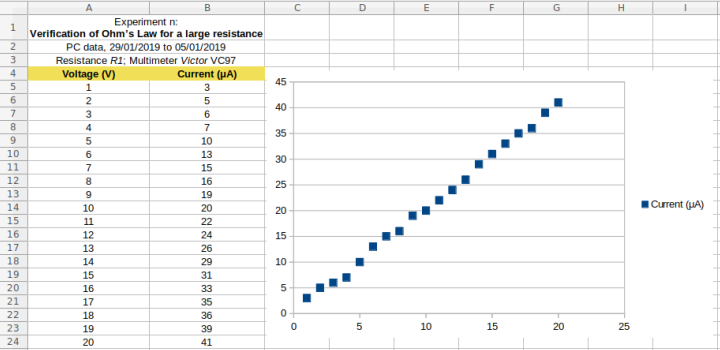
\includegraphics[scale=0.75]{figs/samplegraph1.png}
    \caption{Sample graph of the data in Table (\ref{table:sampledata}) with much to be improved.}
    \label{fig:samplegraph1}
\end{figure}

Excel's biggest user base is business, so default graph formats are mostly setup for that purpose. As a result, changes need to be made to bring it to a `scientific' format: 
\begin{enumerate}
    \item Remove any unnecessary white space. You can do this by adjusting the minimum and maximum values of the axes. You can do this by right clicking the axes and selecting \texttt{Format Axes}.
    
    \item Remove the legend on the right when possible: these are usually just a waste of space. You can select it and press \texttt{Delete}. Any information regarding the graph should be added in the caption.
    
    \item Change the marking icon to a more scientific size and shape. You can right click the graph and select \texttt{Format Data Series} and edit the icon size and shape there.
    
    \item Remove the grid-lines and the tick-marks on the axes.
\end{enumerate}

You should now have a graph like the one shown in Figure (\ref{fig:samplegraph2}).

\begin{figure}[!htb]
    \centering
    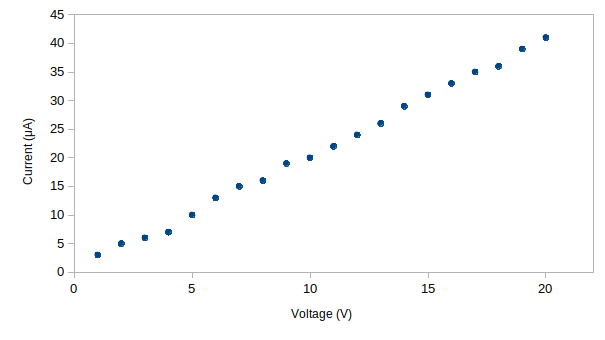
\includegraphics[scale=0.8]{figs/samplegraph2.png}
    \caption{Same graph as in Figure (\ref{fig:samplegraph1}), with some modifications made.}
    \label{fig:samplegraph2}
\end{figure}


\subsubsection{Adding a Trendline}

It should appear to you now that this trend is quite linear. We can now use the computer's algorithm to get the `best' straight line between these points. Don't worry right now about how this is done, you will learn about this in some detail at a later point.

Right-clicking the data-points, select \texttt{Add Trendline}. In the dialog box that opens, choose a \texttt{Linear} regression type and select the checkbox that says \texttt{Show Equation}. You can also make the line dotted, and change its colour. 

If your trendline equation looks something like this:
\begin{center}
    \texttt{f(x) = 0.950310374968518 x - 0.011427047596473}
\end{center}

then edit it to round it off to a more reasonable number of digits. You will understand how many digits is reasonable in the next chapter on error analysis, for right now, let us choose to keep three decimal places. You should now have a graph that looks like Figure (\ref{fig:samplegraph3}).

\begin{figure}[!htb]
    \centering
    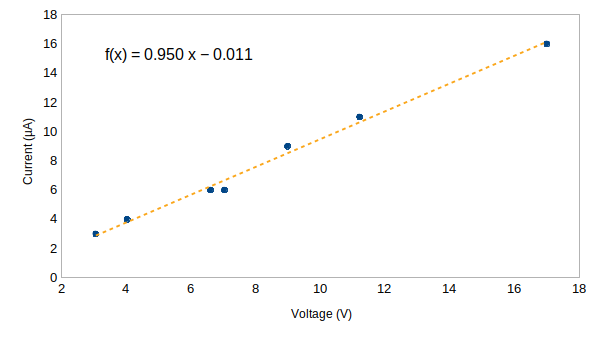
\includegraphics[scale=0.8]{figs/samplegraph3.png}
    \caption{Same graph as in Figure (\ref{fig:samplegraph1}), with formatted trendline.}
    \label{fig:samplegraph3}
\end{figure}

\begin{tip}
In Microsoft Excel, you can make the current graph style a `template', so that you don't have to keep making most of these changes every time you plot new data. To do this, right-click the chart, and select \texttt{Save as Template}. Choose an appropriate name for the chart template and save it. The chart template automatically appears in the \texttt{Templates} folder for charts. You can access it on the \texttt{All Charts} tab in the \texttt{Insert Chart} or \texttt{Change Chart Type} dialog box, where you can apply a chart template like any other chart type.
\end{tip}

\subsection{Graphing with Python}

The purpose of the lab is not to familiarise you to coding with Python -- there is another course that does that. We will be using Python for elementary data analysis. Everything that can be done here can alternatively also be done using Microsoft Excel, so you have a choice of which software to use.



In this section you will learn how to use Python to:

\begin{enumerate}
    \item Import data from CSV files or spreadsheets,
    \item Plot a basic graph,
    \item Add a trendline with its equation.
\end{enumerate}

\subsection{Basic Coding}

As with the other Physics courses, we will be using \textbf{\href{https://jupyter.org}{Jupyter Notebook}}. Go to the link and follow the instruction procedure to install \href{https://www.anaconda.com/downloads}{Anaconda}, a Python distribution that comes with Jupyter pre-installed.

\begin{imp}
The installation of Anaconda Python -- and consequently Jupyter Notebook -- takes a significant amount of time. As a result, you should get it done \textbf{before this session begins}. 
\end{imp}






%\section{Apparatus}



%\section{Description}



%\section{Suggested Procedure}



\newpage